\documentclass[twoside,a4paper,12pt]{book}
\usepackage[twoside,a4paper,top=3.5cm, left=4cm, width=15cm, height=22.5cm]{geometry}
\usepackage[utf8]{inputenc}
\usepackage{graphicx}
\usepackage{float}
\usepackage{appendix}
\usepackage{fancyhdr}
% package for providing the size of columns on tables
\usepackage{array}
\usepackage{color}
% Package for avoiding the issue with the option hidelinks of the package hyperref
\usepackage[colorlinks=true,
            linkcolor=black,
            urlcolor=blue,
            citecolor=black,
            hyperfootnotes=true]{hyperref}
\usepackage{caption}
\usepackage{eurosym}
\usepackage{multirow}
\usepackage{listings}
\usepackage[nohyperlinks,smaller,withpage]{acronym} 
\usepackage{enumitem}
\usepackage[acronym]{glossaries}
\usepackage{mathtools}
\DeclarePairedDelimiter{\ceil}{\lceil}{\rceil}

\newcommand{\ada}[1]{\lstinline[style=ada,
keywordstyle=\mdseries,breaklines,backgroundcolor=\color{white}]&#1&}
\newcommand{\asm}[1]{\lstinline[style=sparc,
keywordstyle=\mdseries,breaklines,backgroundcolor=\color{white}]$#1$}
\newcommand{\prog}[1]{\asm{#1}}

\definecolor{dkgreen}{rgb}{0,0.6,0}
\definecolor{gray}{rgb}{0.8,0.8,0.8}
\definecolor{mauve}{rgb}{0.58,0,0.82}

% json style
\lstset{
    string=[s]{"}{"},
    stringstyle=\color{blue},
    comment=[l]{:},
    commentstyle=\color{black},
}

\lstdefinestyle{c}{
       language=c,
        basicstyle=\footnotesize\ttfamily,
        aboveskip= \bigskipamount,
        belowskip= \bigskipamount,
        abovecaptionskip= \medskipamount,
        belowcaptionskip=\bigskipamount,
        xleftmargin=\parindent,
        columns=flexible
}

\lstdefinestyle{xml}{
       language=xml,
        basicstyle=\sffamily,
        aboveskip= \bigskipamount,
        belowskip= \bigskipamount,
        abovecaptionskip= \medskipamount,
        belowcaptionskip=\bigskipamount,
        xleftmargin=\parindent,
        columns=flexible
}

\makeglossaries


\begin{document}

\newacronym{eboa}{E-BOA}{Engine for Business Operation Analysis}

\newacronym{rdbms}{RDBMS}{Relational Database Management System}

\newacronym{uuid}{UUID}{Universally unique identifier}

\newacronym{pid}{PID}{Process identifier}


\newglossaryentry{leon2}{name={LEON2},
    description={Es un core de microprocesador de 32-bits basado en la
    arquitectura RISC y en el conjunto de instrucciones SPARC V8. Originalmente
    diseñada por la \gls{esa}, y
    posteriormente por Gaisler Research
    }}


\pagestyle{empty}
% -*-front.tex-*-
%
% Cover page for the GSDM documentation
%
% Written by DEIMOS Space S.L. (dibb)
%
% module gsdm

\begin{titlepage}
	
    
\includegraphics[scale=0.20]{../fig/deimos_logo.jpg}
    
    \vspace{2.0cm}
    
    	\begin{center}
    
    \vspace{2cm}
    
    \LARGE{\textbf{GSDM: Ground Segment Data Management}} \\    
    \LARGE{Dynamic data modelling for ground segment data management facilities}
    
    	\end{center}    
    
    \vspace{7.0cm}

    \vspace{0.5cm}

    \Large{\textbf{GSDM release:} 0.1.0}

    \Large{\textbf{Document release:} 1.0}

    \vspace{1cm}
    
    \large{Date: \today}
    
\end{titlepage}

\cleardoublepage

\setcounter{page}{1}
\pagenumbering{roman}

\frontmatter % Introduction, indexes ...

\tableofcontents
\listoffigures
\listoftables

\mainmatter
\pagestyle{fancy}
\fancyhead{}
\fancyhead[RE]{\slshape \rightmark} 
\fancyhead[LO]{\slshape \leftmark}  
\fancyfoot{}
\fancyfoot[C]{\lowercase{\thepage}}

% Introduction
\chapter{Introduction}\label{c:intro}

\acrshort{eboa} is the component aimed to serve as data storage management for business operation analysis. The component aims to allow a dynamic data structure for reducing the effort of developing data models and managing the complex relations between data received.

All the information received is stored into the database using the following high-level entities:

\begin{itemize}

\item Explicit reference: identifier referring to an entity business-related
\item Event: period of time associated to a gauge of a certain aspect business-related
\item Annotation: particular aspect associated to an explicit reference
\item Input: block of information received from the external interface to process. After the processing, the interesting information is extracted and stored inside the system.
\item Alert: notification to users regarding anomalies identified by the system related to previous entities.
\item Report: container of analysis.

\end{itemize}


% Purpose and scope
\chapter{Purpose and scope}

This component manages the storage of the data received following the next requirements:

\begin{itemize} 

\item Traceability of all the data to the source of information (even information created within the infrastructure)

\item No pre-configuration needed for inserting data

\item Include modern datatypes for storing the data

\item Flexible structure for linking information to events and annotations

\item Flexible structure for linking events between them

\item Flexible structure for linking explicit references between them

\item Continuous developtment/Continuous integration approach

\item Include geo-query functionalities

\item Parallel insertion of data using the \acrshort{rdbms} parallelism mechanisms

\item Quick access to the information by which it can be managed dynamically depending on the needs of the users

\end{itemize}

The scope of this component targets systems/tools with the need of storing time-tagged information. The data model used allows quick access to the information in a structured way.


% Data model
\chapter{Data model}

The \acrshort{gsdm} implements the data model shown in the figure \ref{fg:gsdmdb}.

\begin{figure}[ht]
  \begin{center}
	\centering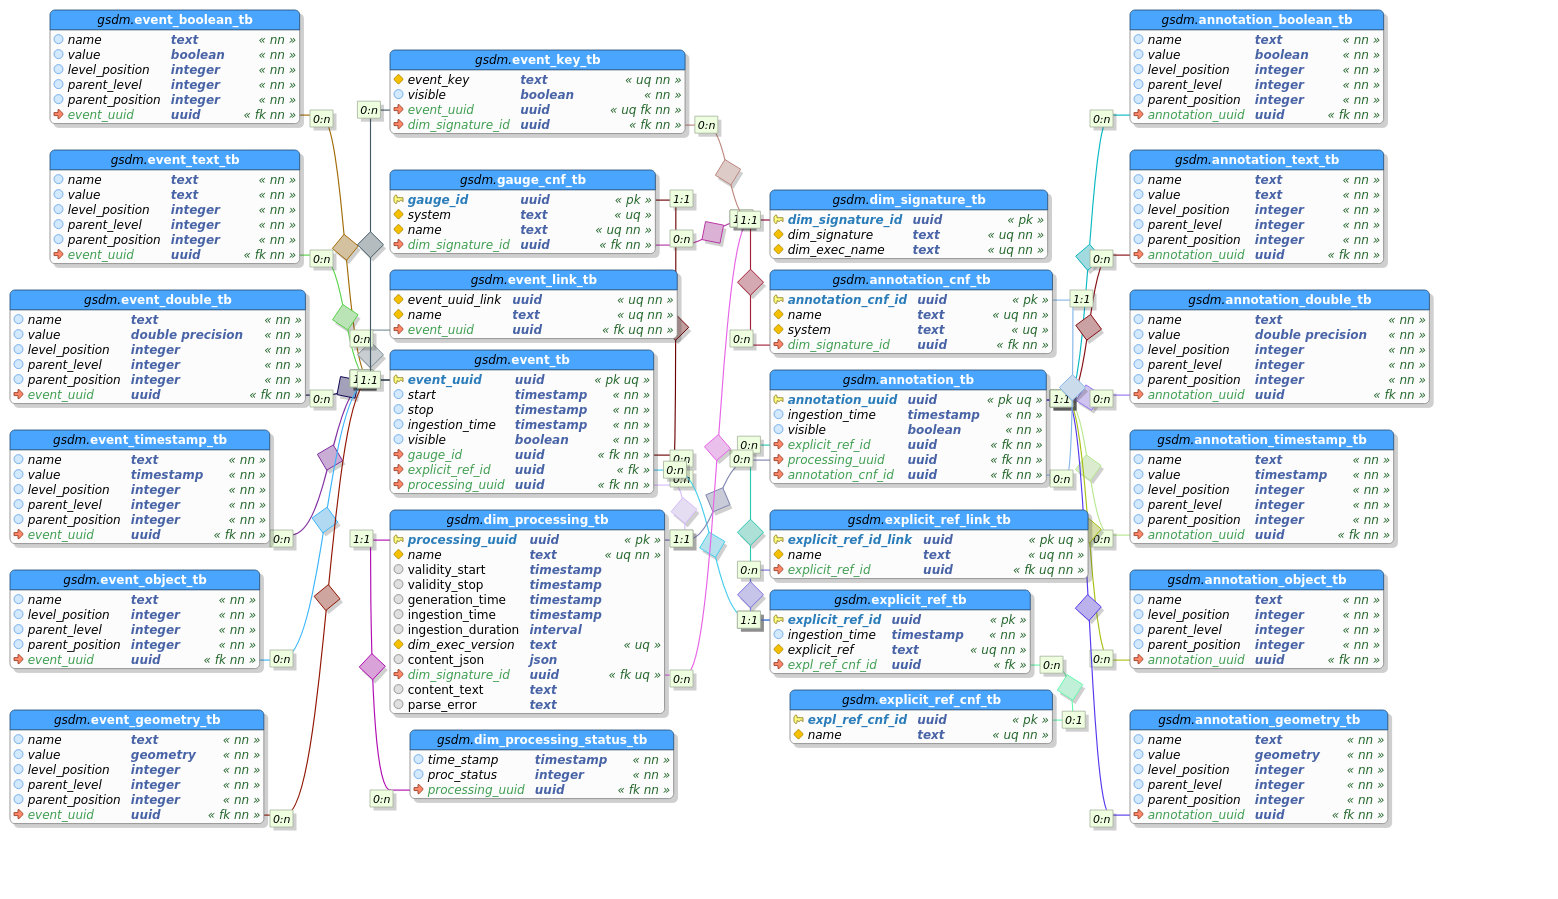
\includegraphics[width=150mm]{../fig/gsdmdb.png}
	\caption{Data model of the \acrshort{gsdm}}
	\label{fg:gsdmdb}
  \end{center}
\end{figure}

As said in chapter \ref{c:intro}, there are 4 main entities in the data model: explicit references (explicit\_ref\_tb), events (event\_tb), annotations (annotation\_tb) and inputs (dim\_processing\_tb).

The entities event and annotation may have an associated dynamic structure of values. These values indicate properties/information of the related entities interesting for the data model. These values are structured in the database following the schema of the figure \ref{fg:values_structure}.

\begin{figure}[ht]
  \begin{center}
	\centering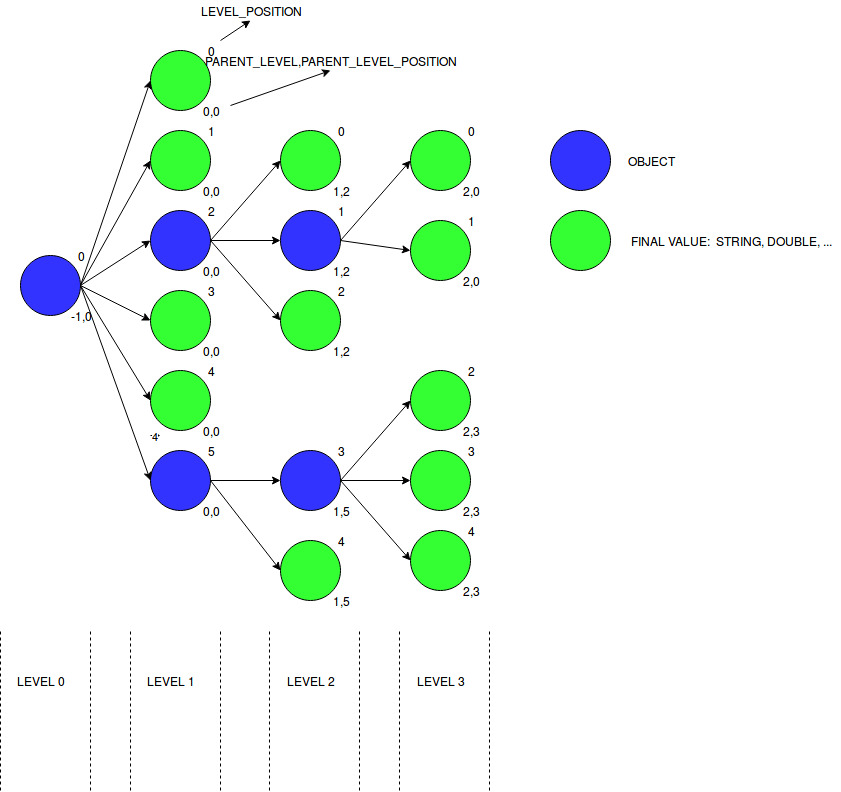
\includegraphics[width=150mm]{../fig/values_structure.jpg}
	\caption{Structure of the values associated to events and annotations}
	\label{fg:values_structure}
  \end{center}
\end{figure}

The values associated to an entity may have one of the following types:

\begin{itemize}

\item Boolean
\item Text
\item Double
\item Timestamp
\item Geometry
\item Object

\end{itemize}

The type object allows every entity to have an associated structure of values (containing other objects). This structure is defined like a tree, every node of the tree may have any of the types described in the previous list. If the node has the type object, the branch has to continue till the final node has a type different than the type object.
The way the tree is structured is as follows:

\begin{enumerate}

\item Every node has a level position
\item Every node has a reference to its parent represented by the parent level and parent level position values
\item Every parent node has the type object
\item Every final node of a branch has a type different than the type object

\end{enumerate}

To better understand how the structure of values is managed by the \acrshort{gsdm}, here it is an example:

Input:
\begin{lstlisting}[breaklines=true, style=xml, caption={XML input example for showing the values structure management.}]
<gsd>
  <insert>
    <dim_signature
        name="test_dim_signature1"
        version="1.0"
        exec="test_exec1"/>
    <source
        name="test_simple_update.xml" 
        generation_time="2018-06-06T13:33:29"
        validity_start="2018-06-05T02:07:03"
        validity_stop="2018-06-05T02:07:36"/>
    <data>
      <event start="2018-06-05T02:07:03"
             stop="2018-06-05T02:07:36"
             key="test_key2"
             explicit_reference="test_explicit_ref2"
             link_ref="event_link_id2">
        <links>
          <link name="test_link_name2" link_mode="by_ref">event_link_id1</link>
        </links>
        <gauge name="test_gauge_name2"
               system="test_gauge_system2"
               insertion_type="SIMPLE_UPDATE"/>
        <values name="test_object_name2">
          <value name="test_text_name2" type="text">test text2</value>
          <value name="test_boolean_name2" type="boolean">true</value>
          <value name="test_double_name2" type="double">0.91234</value>
          <values name="test_object_name3">
            <value name="test_text_name3" type="text">test text2</value>
            <value name="test_geometry2" type="geometry">29.012974905944
            -118.33483458667
            29.012974905944
            -118.33483458667</value>
          </values>
        </values>
      </event>
    </data>
  </insert>
</gsd>
\end{lstlisting}

Output:

\begin{lstlisting}[breaklines=true, caption={JSON output after query the gsdm for the specific event previously shown.}]

{"_sa_instance_state": <sqlalchemy.orm.state.InstanceState object at 0x7f633a920630>,
 "event_uuid": UUID("b271b268-b048-11e8-b1cd-000000006318"),
 "level_position": 0,
 "name": "test_object_name2",
 "parent_level": -1,
 "parent_position": 0}
{"_sa_instance_state": <sqlalchemy.orm.state.InstanceState object at 0x7f633a9304e0>,
 "event_uuid": UUID("b271b268-b048-11e8-b1cd-000000006318"),
 "level_position": 0,
 "name": "test_text_name2",
 "parent_level": 0,
 "parent_position": 0,
 "value": "test text2"}
 {"_sa_instance_state": <sqlalchemy.orm.state.InstanceState object at 0x7f633a9306d8>,
 "event_uuid": UUID("b271b268-b048-11e8-b1cd-000000006318"),
 "level_position": 1,
 "name": "test_boolean_name2",
 "parent_level": 0,
 "parent_position": 0,
 "value": True}
 {"_sa_instance_state": <sqlalchemy.orm.state.InstanceState object at 0x7f633a92b0b8>,
 "event_uuid": UUID("b271b268-b048-11e8-b1cd-000000006318"),
 "level_position": 2,
 "name": "test_double_name2",
 "parent_level": 0,
 "parent_position": 0,
 "value": 0.91234}
 {"_sa_instance_state": <sqlalchemy.orm.state.InstanceState object at 0x7f633a920f60>,
 "event_uuid": UUID("b271b268-b048-11e8-b1cd-000000006318"),
 "level_position": 3,
 "name": "test_object_name3",
 "parent_level": 0,
 "parent_position": 0}
{"_sa_instance_state": <sqlalchemy.orm.state.InstanceState object at 0x7f633a930550>,
 "event_uuid": UUID("b271b268-b048-11e8-b1cd-000000006318"),
 "level_position": 0,
 "name": "test_text_name3",
 "parent_level": 1,
 "parent_position": 3,
 "value": "test text2"}
{"_sa_instance_state": <sqlalchemy.orm.state.InstanceState object at 0x7f633a9303c8>,
 "event_uuid": UUID("b271b268-b048-11e8-b1cd-000000006318"),
 "level_position": 1,
 "name": "test_geometry2",
 "parent_level": 1,
 "parent_position": 3,
 "value": <WKBElement at 0x7f633a9305f8; 01030000000100000037000000bab2cc5252033d404fd40bee6d955dc0b71be99d72dd3c40e4ff1f50cf975dc03fd8f5e298b73c4015a6d00c2f9a5dc00b173561be913c40117082478d9c5dc0142857d6e06b3c40edf52a6fea9e5dc0759e911afe453c40e7807a3247a15dc00b99eda117203c4054bc9b6da3a35dc08e6c65542dfa3b4086b0ab05ffa55dc00fec708441d43b401f266aa959a85dc0c234706521c13b409a546f4e89a95dc02b2990c36dba3b4073ad4aa9bd9e5dc0ef04fb9096b33b40c10d6c571b945dc0a31409a298ac3b40741fa9a29d895dc041ca98b770a53b40f95e32e53f7f5dc04f61ea7e1b9e3b40e3646887fd745dc0f99a399195963b401afbb3fdd16a5dc07c744273db8e3b40382a94c6b8605dc078708094e9863b40816ea968ad565dc0a385764ebc7e3b40d9a80b71ab4c5dc0b04095e34f763b40f7037e71ae425dc01432147ea06d3b4090abc8feb1385dc0f4567d2eaa643b409a170bafb12e5dc0a77c05ea685b3b407b040b18a9245dc092cdc288d8513b40e8ada7cd931a5dc0470088c3f4473b40207f1e606d105dc0606fa831b93d3b40ed827d5a31065dc0e463305321333b404a701f4fdbfb5cc083263eed09273b40166ec11359f05cc04b4176f41e3a3b40edb9b49509ef5cc06ac2ec29f55f3b404c4c24666fec5cc05706f32bc9853b40b5087efcd3e95cc00df5b35597ab3b407c3bfe7737e75cc0e835fedc5fd13b40b92260099ae45cc0f5bb443821f73b403d9452eafbe15cc01b27e9d6dd1c3c403529415a5cdf5cc0028b00fe98423c40975de8d3badc5cc0421be70d5c683c40f30d99ef16da5cc0dd840c8587743c4019d72226bae55cc05b2b8ebc307f3c4073d37b012ef05cc00de2d1c87c893c406f20bea487fa5cc0860fb83b70933c40ee7aeb8ecb045dc00e0d1f9b0f9d3c401d362657fe0e5dc08533ac295fa63c40f0a9496824195dc0d196c11763af3c403ade713a42235dc0171a48771fb83c40de6ab2435c2d5dc0637dc83d98c03c40423d0cfa76375dc00854fc45d1c83c4016f2f5d496415dc060e03f51ced03c408b34164fc04b5dc075a9d20893d83c40d4d6fee7f7555dc01c75cafe22e03c402000de2542605dc086b7ecae81e73c4027645297a36a5dc0dd0f407fb2ee3c408cb137d520755dc0f2359ec0b8f53c40fbecc084be7f5dc05ad5879397fc3c40d08b3635818a5dc0bab2cc5252033d404fd40bee6d955dc0>}
 
\end{lstlisting}

So, all values are associated to the proper level position, parent level and parent level position values.

% Testing environment
\chapter{GSDM testing environment}\label{c:install_gsdm}

Inside the repository of the \acrshort{gsdm} component there is a \href{https://www.vagrantup.com/}{Vagrant} configuration file so that the environment for testing can be created automatically.

For doing so, follow the next steps:

\begin{enumerate}

\item Clone the repository

\begin{lstlisting}[breaklines=true, style=bash]

$ git clone https://bitbucket.org/dbrosnan/gsdm.git

\end{lstlisting}

\item Enter into the repository folder

\begin{lstlisting}[breaklines=true, style=bash]

$ cd (PATH_TO_GSDM)/gsdm

\end{lstlisting}

\item Run vagrant (see installation instructions in the referenced link)

\begin{lstlisting}[breaklines=true, style=bash]

$ vagrant up centos

\end{lstlisting}

\end{enumerate}

This will create a virtual machine with all you need to test the GSDM component.

In order to check that the component has been correctly installed, run the following commands to execute the automated tests:

\begin{lstlisting}[breaklines=true, style=bash]]

$ vagrant ssh centos
$ cd /vagrant/src/
$ py.test -v --cov-report html:tests/tmp/code_coverage_analysis --cov=gsdm tests

\end{lstlisting}

In order to check the coverage report, check Annex 1 and install firefox and open the code coverage analysis report:

\begin{lstlisting}[breaklines=true, style=bash]]

$ sudo yum install firefox
$ firefox tests/tmp/code_coverage_analysis/index.html

\end{lstlisting}

\section {Connecting to vagrant with X11 forwarding}

Read these links for detailed information:

\begin{itemize}

\item \href{https://coderwall.com/p/ozhfva/run-graphical-programs-within-vagrantboxes}{Run graphical programs within Vagrantboxes} 
\item \href{https://www.cyberciti.biz/faq/how-to-fix-x11-forwarding-request-failed-on-channel-0/}{Install X authority file utility} 

\end{itemize}

Allow X-Forwarding in your Vagrantfile:

To use X-Forwarding, you first need to allow it from within your Vagrantfile, like this:

\begin{lstlisting}[breaklines=true, style=bash]]

Vagrant.configure(2) do |config|
  ...
  config.ssh.forward_x11 = true
end

\end{lstlisting}

To be able to execute GUIs in the ssh session, you have to install xauth inside the virtual machine created:

\begin{lstlisting}[breaklines=true, style=bash]]

sudo yum install xauth

\end{lstlisting}

Now on your host run this:

\begin{lstlisting}[breaklines=true, style=bash]]

$ vagrant ssh-config
Host some_site
  HostName 127.0.0.1
  User vagrant
  Port 2222
  UserKnownHostsFile /dev/null
  StrictHostKeyChecking no
  PasswordAuthentication no
  IdentityFile vagrant.d/insecure_private_key
  IdentitiesOnly yes
  LogLevel FATAL
  ForwardX11 yes

\end{lstlisting}

Now you can ssh with X11 forwarding:

\begin{lstlisting}[breaklines=true, style=bash]]

ssh -X -p 2222 vagrant@localhost -i vagrant.d/insecure_private_key

\end{lstlisting}



% Create ingestion processor
\chapter{Create ingestion processor}

In the following chapter, the process of creating a processor for ingesting data to the \acrshort{eboa} module is explained.

The explanation is based on an example for ingesting Sentinel-2 data from the planning system (data received on NPPF files, xml formatted).

The example will use the python interface of the component, as the target version of the \acrshort{eboa} used in this explanation is the 0.1.0 and it is the only interface available.

\section{Installing EBOA on vagrant}

See the details in section \ref{c:install_eboa}.

\section{Structure of the folders and location of ingestion processors inside the project}

The ingestion processors are being located for the moment in the folder:

\begin{lstlisting}[breaklines=true, style=bash]]

src/ingestions

\end{lstlisting}

Inside this folder there is the folder s2 where the example explained here can be located:

\begin{lstlisting}[breaklines=true, style=bash]]

src/ingestions/s2/ingestion_nppf

\end{lstlisting}

There, the code of the processor, a folder for automated tests and a folder for input examples can be found:

\begin{lstlisting}[breaklines=true, style=bash]]

ingestion_nppf.py
input_files
tests

\end{lstlisting}

It is recommended to read the code inside the file ingestion\_nppf.py.

\section{Processor code}

For creating ingestion processors the \acrshort{eboa} component offers some helpers through the submodule ingestion which can be seen in the section \ref{\detokenize{eboa.ingestion:module-eboa.ingestion.functions}}.

The processor code has a main method:

\begin{lstlisting}[breaklines=true, style=python]]
def process_file(file_path):
    """Function to process the file and insert its relevant information
    into the DDBB of the eboa

    :param file_path: path to the file to be processed
    :type file_path: str
    """
\end{lstlisting}

Which should be provided as interface of the processor as in future versions it will be the main entry point to the processor.

This method shall extract from the file passed by parameter all the interesting information to the system.

The data extracted has to be formatted with the structure of a python dictionary which can be validated against a schema implemented in the engine side of the \acrshort{eboa} (method eboa.engine.engine.validate\_data). This data will be validated before treatement by the engine.

An example of the data structure, that has to follow the data to be inserted into the \acrshort{eboa}, can be seen in appendix \ref{ap:example_data_structure}.

For the version of this example of an ingestion processor, this method is called from the same phyton file from another method that is called from the main entry point to the file:

\begin{lstlisting}[breaklines=true, style=python]]
def command_process_file(file_path):
    # Process file
    data = process_file(file_path)
    ...

if __name__ == "__main__":
    ...

    returned_value = command_process_file(file_path)
\end{lstlisting}

Once the data has been extracted the method command\_process\_file(file\_path) will interface with the Engine of the \acrshort{eboa} to insert the data:

\begin{lstlisting}[breaklines=true, style=python]]
    # Process file
    data = process_file(file_path)

    engine = Engine()
    # Validate data
    filename = os.path.basename(file_path)

    # Treat data
    returned_value = insert_data_into_DDBB(data, filename, engine)
\end{lstlisting}

\section{Extraction of data}

\subsection{Extraction from an XML file}

The example provided performs the extraction of data from an XML file. To do so, the module uses the library \href{https://pypi.org/project/lxml/}{lxml}.

The following list includes a brief description of main operations available using this library:

\begin{itemize}
\item Importing the module:
\begin{lstlisting}[breaklines=true, style=python]]
# Import xml parser
from lxml import etree
\end{lstlisting}
\item Obtain Xpath object for reading the XML using XML paths:
\begin{lstlisting}[breaklines=true, style=python]]
    file_name = os.path.basename(file_path)
    parsed_xml = etree.parse(file_path)
    xpath_xml = etree.XPathEvaluator(parsed_xml)
\end{lstlisting}
\item Get nodes of an XML:
\begin{lstlisting}[breaklines=true, style=python]]
    record_operations = xpath_xml("/Earth_Explorer_File/Data_Block/List_of_EVRQs/EVRQ[RQ/RQ_Name='MPMMRNOM' or RQ/RQ_Name='MPMMRNRT']")
\end{lstlisting}
\item Perform operations with one node:
\begin{lstlisting}[breaklines=true, style=python]]
    generation_time = xpath_xml("/Earth_Explorer_File/Earth_Explorer_Header/Fixed_Header/Source/Creation_Date")[0].text.split("=")[1]
\end{lstlisting}
\end{itemize}

\section{Manual execution of the processor}

The processor can be manually executed passing the file path to be processed as follows:

\begin{lstlisting}[breaklines=true, style=bash]]

$ cd /vagrant/src/ingestions/s2/ingestion_nppf
$ python3 ingestion_nppf.py -f input_files/S2B_OPER_MPL__NPPF__20180727T110000_20180813T140000_0001.EOF

\end{lstlisting}

\section{Automated tests}

Inside the folder tests, there should be a python file which would cover the unit testing of the processor. For the example explained in this page, to execute the tests, run the following command:

\begin{lstlisting}[breaklines=true, style=bash]]

$ cd /vagrant/src/ingestions/s2/ingestion_nppf
$ py.test -v --cov-report html:tests/tmp/code_coverage_analysis --cov=ingestions tests/

\end{lstlisting}

Then, the code coverage analysis may be checked (following the instructions shown in the section \ref{x11_forwarding} and installing firefox) with the following command:

\begin{lstlisting}[breaklines=true, style=bash]]

$ firefox tests/tmp/code_coverage_analysis/index.html

\end{lstlisting}

\subsection{Creating the tests}

For validating the correct behaviour of the ingestion processor, automated tests should be provided which would cover completely the code of the ingestion processor.

For doing this, the provided solution makes use of the library unittest. With this library the utility py.test can detect all the tests inside a project, execute them and provide analysis on the failures.

The following list includes a brief description of main operations available using this library:

\begin{itemize}
\item Import the module:
\begin{lstlisting}[breaklines=true, style=python]]
import unittest
\end{lstlisting}
\item Define class for testing:
\begin{lstlisting}[breaklines=true, style=python]]
class TestEngine(unittest.TestCase):
\end{lstlisting}
\item Define the main method which will be executed every time before a unit test is executed:
\begin{lstlisting}[breaklines=true, style=python]]
    def setUp(self):
        # Create the engine to manage the data
        self.engine_eboa = Engine()
        self.query_eboa = Query()

        # Create session to connectx to the database
        self.session = Session()

        # Clear all tables before executing the test
        for table in reversed(Base.metadata.sorted_tables):
            engine.execute(table.delete())
\end{lstlisting}
\item Define unit tests:
\begin{lstlisting}[breaklines=true, style=python]]
    def test_insert_insert_nppf(self):
        filename = "NPPF_CONTAINING_ALL_DATA_TO_BE_PROCESS.EOF"
        file_path = os.path.dirname(os.path.abspath(__file__)) + "/inputs/" + filename

        ingestion.command_process_file(file_path)

        # Check that events before the queue deletion are not inserted
        events_before_validity_period = self.session.query(Event).filter(Event.stop < "2018-07-20T13:40:00.000").all()

        assert len(events_before_validity_period) == 0
\end{lstlisting}
\end{itemize}


\begin{appendices}

\chapter{Why UUIDs as primary keys instead of auto-increment IDs?}

Designs of relational databases must have a secure out of conflicts way of identifying entities inside the database. One possible solution for this is using auto-increment functions of the database to provide this secure out of conflicts way of identifying entities.

Using the auto-increment functions, though, implies a huge problem: the information has to be inserted in a sequential way so that the foreign keys are built by the database manager (PostgreSQL in this case).

A solution implemented in the data model of the \acrshort{gsdm} is using \acrshort{uuid}s (version 1).

The version 1 of the UUID (according to RFC 4122) is composed by the following fields: 

\begin{lstlisting}[style=bash, caption={XML input example for showing the values structure management.}]

        time_low                the first 32 bits of the UUID
        time_mid                the next 16 bits of the UUID
        time_hi_version         the next 16 bits of the UUID
        clock_seq_hi_variant    the next 8 bits of the UUID
        clock_seq_low           the next 8 bits of the UUID
        node                    the last 48 bits of the UUID

        time                    the 60-bit timestamp
        clock_seq               the 14-bit sequence number
        
\end{lstlisting}

Where the implementation of Python of this version according to the RFC is thread safe due to the following code:

\begin{lstlisting}[style=python, caption={Python code showing how the algorithm provides a mechanism for using UUIDs in a thread safe manner.}]

    global _last_timestamp
    import time
    nanoseconds = int(time.time() * 1e9)
    # 0x01b21dd213814000 is the number of 100-ns intervals between the
    # UUID epoch 1582-10-15 00:00:00 and the Unix epoch 1970-01-01 00:00:00.
    timestamp = int(nanoseconds/100) + 0x01b21dd213814000
    if _last_timestamp is not None and timestamp <= _last_timestamp:
        timestamp = _last_timestamp + 1
    _last_timestamp = timestamp
    
\end{lstlisting}

As \_last\_timestamp is global, this is visible to all the threads of the same process so that they will never see the same timestamp value.

But, this is still not multiprocessing safe. For making the UUIDs creation multiprocessing safe, the UUID has been enforced with the \acrshort{pid} of the process as the "node" field and a random number as the "clock\_seq".

So, this characteristic joint with the addition of the PID warranties the uniqueness of the UUIDs generated inside the GSDM.


\end{appendices}

\backmatter 

\clearpage

\printglossary[type=\acronymtype]

\printglossary

\clearpage

\end{document}
